\chapter{DISPERSI\'ON EL\'ASTICA}\label{dispersionelastica}
\lettrine[lines=3, loversize=-0.1, lraise=0.1]C\ uando estudiamos interacciones electromagn\'eticas, podemos utilizar con gran \'exito la ecuaci\'on de Schr\"odinger para describir sistemas at\'omicos y moleculares porque se puede conocer el Hamiltoniano de interacci\'on en cada caso. Sin embargo, si queremos aplicar esta ecuaci\'on a la descripci\'on de sistemas nucleares o, m\'as general,   a la interacci\'on entre  part\'iculas elementales, la primera dificultad de importancia con la que tropezamos, es que las interacciones entre ellas no son necesariamente electromagn\'eticas, tambi\'en pueden existir interacciones fuertes o d\'ebiles, cuya descripci\'on est\'a dada por las teor\'ias de la cromodin\'amica cu\'antica y electrod\'ebil que en algunas ocasiones, cuando el momento transferido en la colisi\'on es bajo, pueden presentar resultados divergentes y por ende una descripci\'on inadecuada de la din\'amica de la colisi\'on.\\ 

\sp Dado que las part\'iculas elementales son extremadamente diminutas, el \'unico m\'etodo de exploraci\'on que hay para investigar la din\'amica de sus interacciones y su dependencia de
los diversos par\'ametros (energ\'ia, momento orbital,
espines, distancias relativas, etc.), consiste en hacer colisionar part\'iculas y hacer el
subsecuente an\'alisis de los resultados de la interacci\'on ocurrida en circunstancias
controladas.  Por ejemplo, \'este fue el m\'etodo utilizado por Rutherford en los trabajos que culminaron con el establecimiento del modelo at\'omico. Este
ejemplo es importante porque muestra que mediante experimentos de dispersi\'on
de part\'iculas debido a centros dispersores conocidos podemos no s\'olo averiguar la naturaleza y particularidades de la interacci\'on, sino tambi\'en, lo que es muy importante, determinar la estructura de los elementos involucrados en el proceso dispersivo. As\'i, por
ejemplo, fue posible averiguar la estructura electromagn\'etica de los nucleones,
bombarde\'andolos con part\'iculas cargadas \cite{luisdelapeya}. \\

\sp Un proceso de dispers\'ion puede ser de tipo el\'astico o inel\'astico. En el primer caso, las part\'iculas (protones para nuestro trabajo) quedan intactas despu\'es de una colisi\'on, sufriendo una peque\~na desviaci\'on con respecto a sus trayectorias iniciales pero  manteniendo la magnitud de su momento inicial y conservando todos sus n\'umeros cu\'anticos \cite{carlosavila}. En el segundo caso, el estado interno de las part\'iculas se modifica, pueden darse fen\'omenos de excitaci\'on o ionizaci\'on, transformaci\'on
de unas part\'iculas en otras, creaci\'on de nuevas part\'iculas como resultado de la
colisi\'on. Para el desarrollo de este trabajo nos enfocaremos \'unicamente en los procesos el\'asticos.
\section{Estudio de dispersi\'on desde mec\'anica cl\'asica}
Cuando una part\'icula incide sobre un centro dispersor ubicado en el origen de coordenadas (podr\'ia ser un prot\'on
disparado contra un n\'ucleo pesado) con energ\'ia $E$ y par\'ametro de impacto $b$, \'esta se desv\'ia de su trayectoria inicial
con un \'angulo de dispersi\'on $\theta$ (Fig. \ref{figura3})\footnote{Se supone por simplicidad que el objetivo es
azimutalmente sim\'etrico, por lo que la trayectoria permanece en un plano, y que el objetivo
es muy pesado, por lo que el retroceso de este es despreciable.}. El par\'ametro de impacto $b$ es la distancia perpendicular entre la trayectoria de la part\'icula y el eje $z$ que pasa por el centro dispersor \cite{griphys}.
\begin{figure}[H]
%\centering
\begin{tabular}{p{7cm}p{7.45cm}}
\begin{minipage}[l]{7cm}
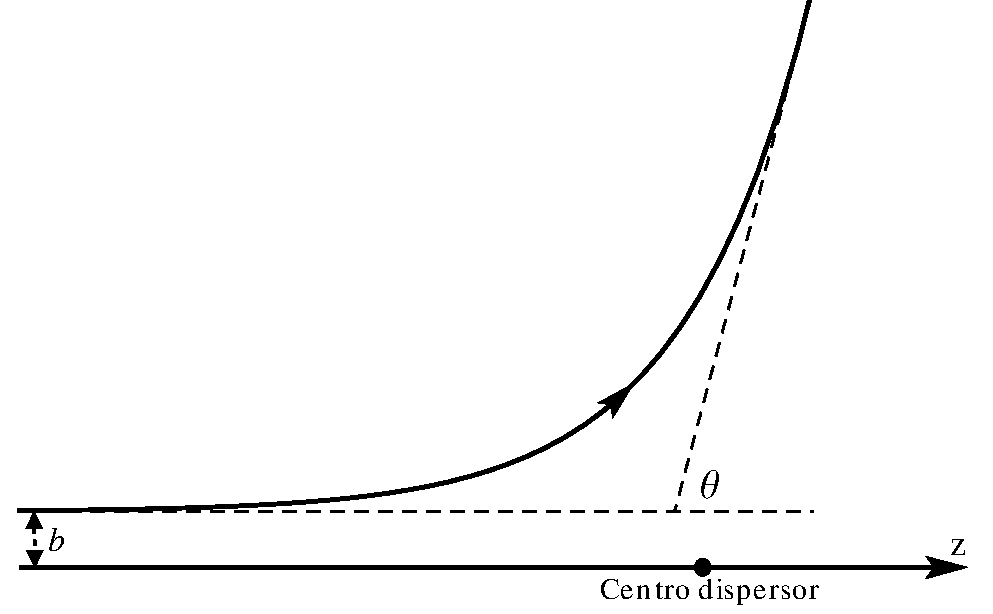
\includegraphics[width=7cm]{Imagenes/figurastesis/dispersor.pdf}
\caption{Dispersi\'on cl\'asica, con par\'ametro de impacto $b$ y \'angulo de disperi\'on $\theta$.}\label{figura3}
\end{minipage}
&
\begin{minipage}[r]{7.45cm}
De modo m\'as general, si un haz de  part\'iculas incide dentro de un  \'area infinitesimal $d\sigma$, este ser\'a dispersado en un correspondiente \'angulo s\'olido infinitesimal \textit{$d\Omega$} (Fig. \ref{figura4}). Cuanto m\'as grande sea $d\sigma$, mayor ser\'a $d\Omega$; El factor de proporcionalidad $D(\theta)\equiv \frac{d\sigma}{d\Omega}$, se denomina secci\'on eficaz diferencial:
\begin{equation}
d\sigma=D\theta d\Omega
\end{equation}
%\end{nuevacaja}
\end{minipage}
\end{tabular}
\end{figure}
En t\'erminos del par\'ametro de impacto y del \'angulo azimutal $\phi$, $d\sigma=bdbd\phi$ y
$d\Omega = \textup{sen}\theta d\theta d\phi$, as\'i:
\begin{equation}
D(\theta)=\frac{b}{\textup{sen} \theta}\left|\frac{db}{d\theta}\right|
\end{equation}
El valor absoluto se debe a que $\frac{db}{d\theta}$ siempre ser\'a negativo\footnote{Porque cuando $b$ crece el \'angulo de dispersi\'on $\theta$ se hace m\'as peque\~no}, esto contradice  la unidad de medida de la secci\'on eficaz (barn $=$ 10$^{-24}$ cm$^2$), el cual corresponde a una unidad de \'area, no puede ser negativa. Por otro lado, $0\leqslant\theta\leqslant\pi$, luego, $\textup{sen} \theta\geqslant 0$. 
\begin{figure}[H]
%\centering
\begin{tabular}{p{9cm}p{5.45cm}}
\begin{minipage}[l]{9cm}
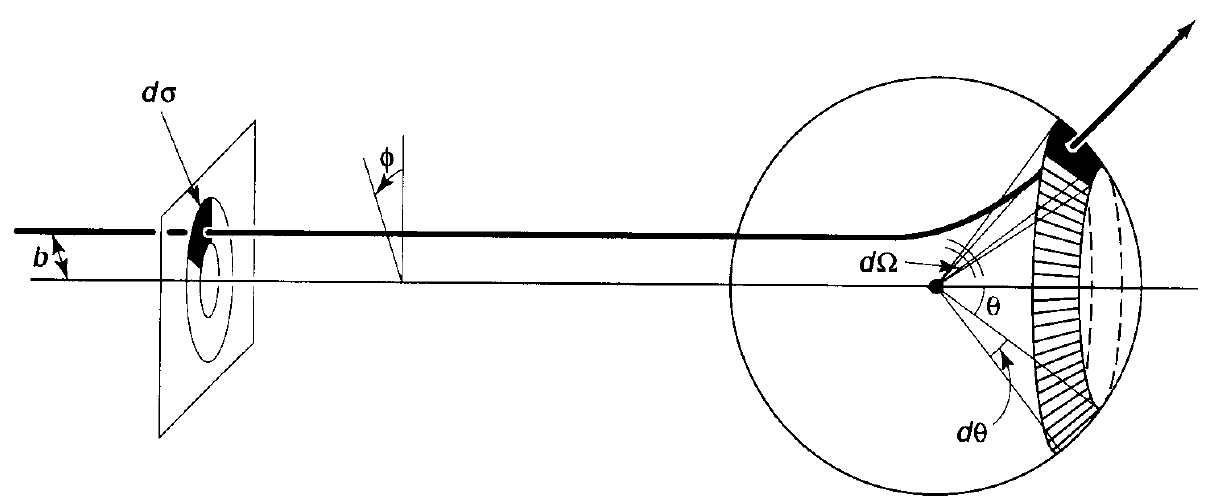
\includegraphics[width=9cm]{Imagenes/figurastesis/angulosolido}
\caption{Part\'iculas que inciden en una peque\~na \'area $d\sigma$ y son desviadas en un \'angulo s\'olido $d\Omega$ \cite{griphys}.}
\label{figura4}
\end{minipage}
&
\begin{minipage}[r]{5.45cm}
La secci\'on eficaz total ($\sigma$) es la integral de $D (\theta)$ sobre todos los \'angulos s\'olidos:
\begin{equation}
\sigma=\int D(\theta)d\Omega,
\end{equation}
y es el \'area transversal total del haz incidente que es dispersado por el blanco.
\end{minipage}
\end{tabular}
\end{figure}
 Por ejemplo, si el centro dispersor es una esfera solida de radio $R$, la secci\'on eficaz total es, $\sigma=\pi R^2$. Que es justamente el \'area transversal de la esfera.
\section{Tratamiento cu\'antico de dispersi\'on}\label{seccion2_2}
En mec\'anica cu\'antica ya no se habla de part\'iculas si no de funciones de onda que describen el estado de la part\'icula. por lo tanto, cuando una onda plana incide sobre un potencial dispersor (sim\'etricamente esf\'erico en $\phi$),  el resultado como consecuencia de esta interacci\'on es una onda esf\'erica, la funci\'on que describe este proceso en la regi\'on asint\'otica\footnote{Por ejemplo, en las proximidades del detector el cual se encuentra ubicado a algunos metros desde donde se presenta la interacci\'on o colisi\'on} ($r\rightarrow \infty$) puede escribirse como el producto de la funci\'on radial asint\'otica $R(r)=e^{ikr}/r$ por una funci\'on angular $f(\theta)$, m\'as la funci\'on de onda plana incidente \cite{griphys,varone}, esto es :
\begin{equation}
\psi(r,\theta)=A \left[ e^{ikz}+f(\theta)\frac{e^{ikr}}{r}\right],
\end{equation}
donde $k=\sqrt{2mE}/\hslash$ es el momento de la onda incidente o dispersada (en procesos el\'asticos, la magnitud del momento antes y despu\'es de la colisi\'on es el mismo), $A$ es la usual constante de normalizaci\'on, $r=\sqrt{x^2+y^2+z^2}$ es la distancia entre el centro dispersor y un frente de onda cualquiera dispersado, $z$ hace referencia a la direcci\'on de propagaci\'on de la onda plana, $f(\theta)$ es la amplitud de dispersi\'on, y contiene toda la informaci\'on acerca del proceso de colisi\'on.\\

\sp Por otro lado, la probabilidad de que  un haz de part\'iculas incidentes pase a trav\'es de un \'area infinitesimal $d\sigma$, es igual a la probabilidad de que el haz de part\'iculas sea dispersado un \'angulo s\'olido infinitesimal $d\Omega$ (para mejor claridad  puede tambi\'en referirse a la figura \ref{figura4}), en consecuencia, 
la secci\'on eficaz diferencial el\'astica en mec\'anica cu\'antica es \cite{griphys}:
\begin{equation}\label{ecu2_6}
\frac{d\sigma}{d\Omega}=\left.|f(\theta)\right.|^2
\end{equation}
 De modo que para conocer la secci\'on eficaz diferencial el\'astica, basta con calcular la expresi\'on para $f(\theta)$ usando la ecuaci\'on de Schr\"odinger. Existen diferentes m\'etodos para determinar la amplitud de dispersi\'on, por lo que solo hablaremos de uno en particular, en el cual est\'an basados los modelos fenomenol\'ogicos descritos en esta tesis. La t\'ecnica se conoce como {\bf an\'alisis de ondas parciales}, y proporciona una expresi\'on exacta para $f(\theta)$.
\section{Desarrollo en ondas parciales}\label{seccion2_3}
La idea b\'asica del m\'etodo de ondas parciales, consiste en
descomponer la funci\'on $f(\theta)$ en una suma infinita, donde cada uno de cuyos t\'erminos est\'a
asociado a un valor definido del momento orbital $l$.\\

Para un potencial de interacci\'on  con simetr\'ia esf\'erica $V(r)$, la ecuaci\'on de Schr\"odinger admite las soluciones separables de la forma $\psi(r,\theta,\phi)=R(r)Y^m_l(\theta,\phi)$, donde $Y^m_l(\theta,\phi)$ es un arm\'onico esf\'erico, y la ecuacion radial viene dada por:
\begin{equation}
-\frac{\hbar^2}{2m}\frac{d^2u}{dr^2}+\left[V(r)+\frac{\hbar^2}{2m}\frac{l(l+1)}{r^2}\right]u=Eu
\end{equation}
donde $u=R(r)/r$ \cite{griphys}.
\begin{figure}[H]
%\centering
\begin{tabular}{p{6cm}p{4cm}}
\begin{minipage}[l]{6cm}
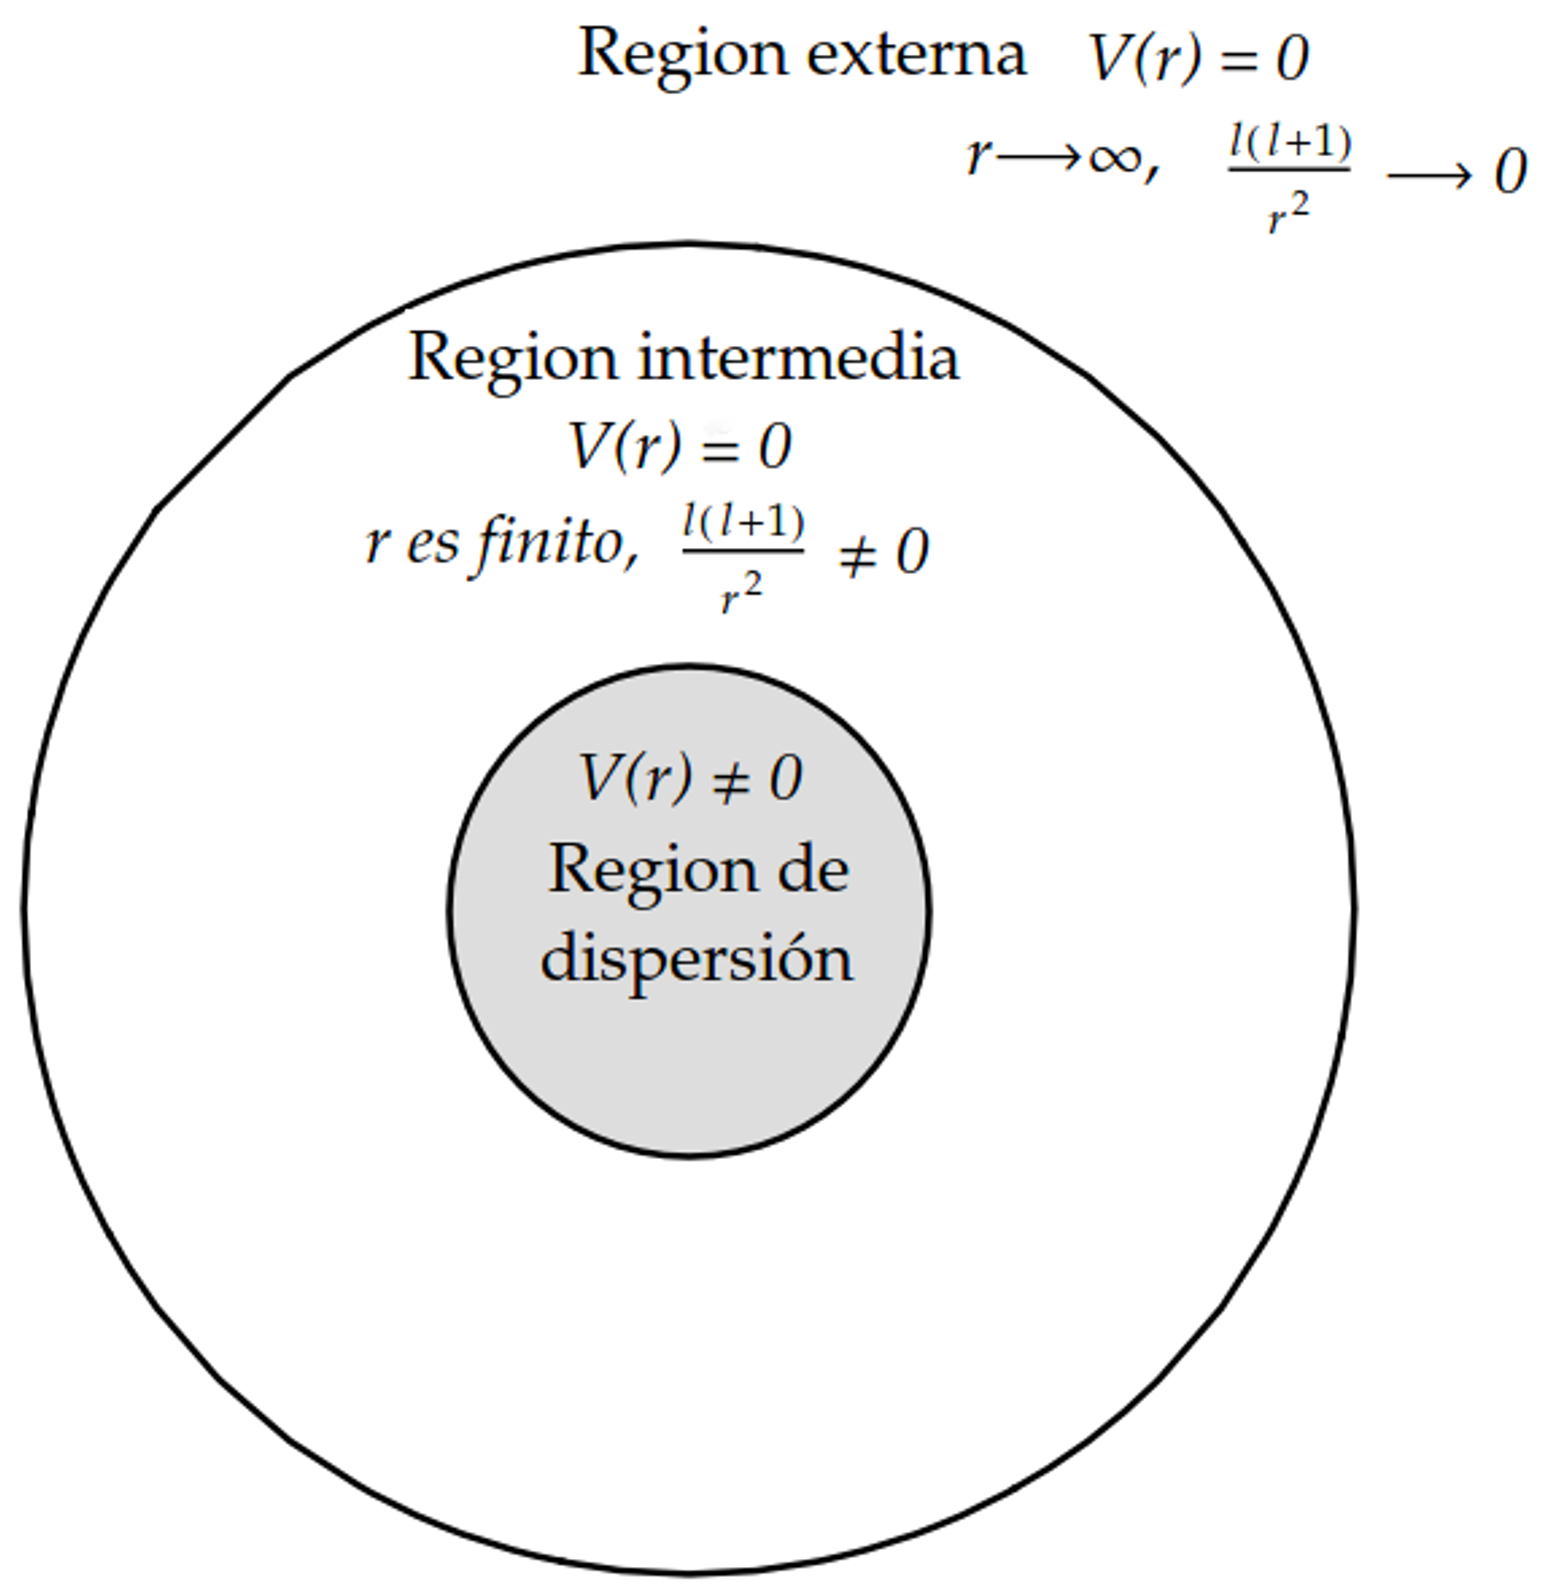
\includegraphics[width=6cm]{Imagenes/figurastesis/potencial.png}
\caption{La figura muestra un potencial dispersor localizado. En la regi\'on de dispersi\'on (sombreado oscuro) el potencial es diferente de cero, en la regi\'on intermedia $V(r)$ puede ser ignorado pero el t\'ermino del momento angular orbital no puede ignorarse, y en la regi\'on externa tanto el t\'ermino del momento angular orbital como el potencial pueden ignorarse.}
\label{figura5}
\end{minipage}
&
\begin{minipage}[r]{8.45cm}
Cuando la interacci\'on se debe a un potencial dispersor de corto alcance, podemos considerarlo como si estuviera contenido en su totalidad en el interior de una esfera de radio finito $R$ (sombreado oscuro en la Fig. \ref{figura5}), por lo que para distancias entre el proyectil
y el blanco mayores que el alcance $R$, el movimiento es libre. Por lo tanto, en la regi\'on externa, donde $r\rightarrow \infty$, $V(r)\rightarrow 0$, y la contribuci\'on del termino del momento angular orbital  es insignificante, luego,
$
R(r)\sim \frac{e^{ikr}}{r}
$ \cite{luisdelapeya}.\\

\sp En la regi\'on intermedia $V(r) = 0$, pero el t\'ermino de momento angular orbital no puede ignorarse,
en consecuencia,  $R(r)\sim h^{(1)}_l(kr)$, donde $h^{(1)}_l(kr)$
son las {\bf funciones esf\'ericas de  Hankel} de primer orden.\\

\sp As\'i, la soluci\'on general exacta a la ecuaci\'on de Schr\"odinger, para un potencial con simetr\'ia azimutal (por tanto independiente del \'angulo $\phi$), fuera de la regi\'on de dispersi\'on, donde $ V (r) = 0$, es \cite{varone}:
\end{minipage}
\end{tabular}
\end{figure}
\begin{equation}\label{ecu2_7}
\psi(r,\theta)=A\left[  
e^{ikz}+k\sum^{\infty}_{l=0}i^{l+1}(2l+1) a_{l}h^{(1)}_l(kr)P_l(\cos\theta)
\right],
\end{equation}
donde\begin{equation}\label{amplituddeondaparcial}
a_l(k)=\frac{e^{2i\delta_l(k)}-1}{2ik},
\end{equation} es la amplitud de la $l-\'esima$ onda parcial y puede ser determinada a partir del  corrimiento de fase de $\delta_l(k)$ de la onda parcial con momento orbital $l$. $P_l(\cos\theta)$ son los polinomios de Legendre. El primer t\'ermino en la ecuaci\'on (\ref{ecu2_7}) representa la onda plana incidente, y la suma, la onda dispersada \cite{griphys}.\\

\sp Por otra parte, los detectores que miden el \'angulo de dispersi\'on est\'an ubicados a distancias muy lejanas, comparadas con el rango de alcance del potencial del centro dispersor, garantizando que la observaci\'on de las part\'iculas dispersadas se hace para r muy grande. En base a este argumento, la funci\'on de Hankel $h_l^{(1)(kr)}$ se aproxima a $(-i)^{l+1}e^{ikr}/kr$ \cite{griphys}. De este modo la funci\'on $\psi(r,\theta)$ es:
\begin{equation}
\psi(r,\theta)\approx A\left[e^{ikz}+f(\theta)\frac{e^{ikr}}{r}\right]
\end{equation}
donde 
\begin{equation}\label{ecufdetheta}
f(\theta)=\sum^{\infty}_{l=0}(2l+1) a_{l}(k)P_l(\cos\theta)
\end{equation}
(Los c\'alculos que lleva a estos resultados pueden hallarse en cualquiera de las referencias \cite{luisdelapeya,griphys}.)
\section{Variables de  Mandelstam}
En las secciones precedentes hemos visto algunos conceptos de la teor\'ia de la dispersi\'on el\'astica de part\'iculas en la representaci\'on de coordenadas y en la descripci\'on que arroja la ecuaci\'on Schr\"odinger. Sin embargo, en colisiones de part\'iculas de alta energ\'ia, es \'util introducir  un tipo de variables cinem\'aticas que son invariantes bajo transformaciones de Lorentz, las variables de  Mandelstam.
\subsection*{Proceso de dos cuerpos}
Para un proceso el\'astico 
\begin{equation}\label{ecu2_12}
A+B\rightarrow A+B,
\end{equation}
con $A$ considerada como part\'icula proyectil y $B$ la part\'icula blanco. Las variables de de  Mandelstam se definen como: 
\begin{align}\label{ecuacion2_13}
s &\equiv (p_{iA}+p_{iB})^2\\
t &\equiv (p_{fA}-p_{iA})^2\\
u &\equiv (p_{fB}-p_{iA})^2
\end{align}
donde $p_{iA}$, $p_{iB}$ son los cuadrimomentos iniciales y 
$p_{fA}$, $p_{fA}$ los cuadrimomentos finales. \\

\sp Usando las definiciones (3.12 - 3.14) y la conservaci\'on de la energ\'ia y momento $p_{iA}+p_{iB}=p_{fA}+p_{fB}$ se tiene que (Ap\'endice C) \cite{varone}:
\begin{equation}\label{ecu2_16}
s+t+u=\sum^4_{i=1}m^2_{i}.
\end{equation}
Para part\'iculas de masas iguales, $\sum^4_{i=1}m^2_i=4m^2$, obtenemos:
\begin{equation}\label{ecu2_16}
s+t+u=4m^2\, \ \ \textup{(s\'olo para part\'iculas de masas iguales)}.
\end{equation}
A cada una de las variables mencionadas ($s$, $t$, $u$) se le asocia un tipo de reacci\'on llamado canal (Fig. \ref{figcanales}).  En el canal $s$ (Fig. \ref{figcanales}a), $t$ es el cuadrado del cuadrimomento\newpage transferido y $s$ es el cuadrado de la energ\'ia total, ambas variables medidas con  respecto al centro de masa (CM). An\'alogamente, en los canales $t$, $u$, las variables $t$, $u$ son el cuadrado de la energ\'ia total del CM.\\

\sp De las tres  variables  invariantes de Lorentz $s$, $t$ y $u$, solo dos de estas son independientes\footnote{Por lo general se toma $s$ y $t$ como variables  independientes} y adem\'as,  suficientes par describir el proceso (\ref{ecu2_12}). Por otro lado, $u$ puede ser expresada en t\'erminos de las variables $s$ y $t$, mediante la ecuaci\'on (\ref{ecu2_16}).
\begin{figure}[H]
%\centering
\begin{tabular}{p{4.816cm}p{4.816cm}p{4.816cm}}
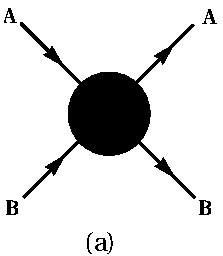
\includegraphics[width=4.23cm]{Imagenes/figurastesis/canalS.pdf} 
\begin{center}
$A+B\rightarrow A+B$
\end{center}
&%division 1-2
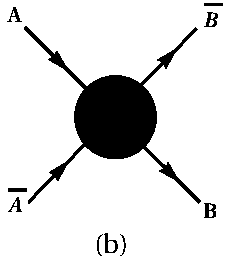
\includegraphics[width=4.23cm]{Imagenes/figurastesis/canalT.pdf}
\begin{center}
$A+\xoverline{A}\rightarrow \xoverline{B}+B$
\end{center}
&%division 2-3
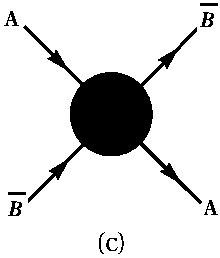
\includegraphics[width=4.23cm]{Imagenes/figurastesis/canalU.pdf}
\begin{center}
$A+\xoverline{B}\rightarrow \xoverline{B}+A$
\end{center}
\end{tabular}
\caption{(a) canal $s$. (b) canal $t$. (c) canal $u$}
\label{figcanales}
\end{figure}
En la figura \ref{figcanales}, $\xoverline{A}$ es la antipart\'iula de $A$ y $\xoverline{B}$ la antipart\'icula de $B$.
\subsection*{Variables s, t y u en el sistema centro de masa (CM)}
\begin{figure}[H]
%\centering
\begin{tabular}{p{5cm}p{4cm}}
\begin{minipage}[l]{5cm}
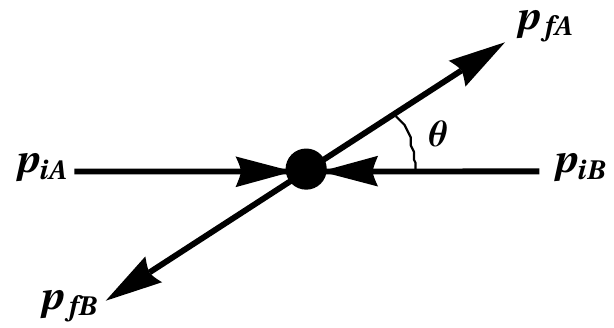
\includegraphics[width=4.6cm]{Imagenes/figurastesis/sistemaCM.png}
\caption{El sistema centro de masa, $\theta$ es el \'angulo de dispersi\'on.}
\label{figsistemaCM}
\end{minipage}
&
\begin{minipage}[r]{9.45cm}
Para una reacci\'on en el canal $s$ (Ecuaci\'on \ref{ecu2_12}). En el sistema CM (Fig. \ref{figsistemaCM}) tenemos por definici\'on:
\begin{equation}\label{ecu2_17}
{\pmb p}_{iA}+{\pmb p}_{iB}=0\ \ \ \textup{(respecto del CM)}
\end{equation}
Los vectores $\pmb{p}_{iA}$  y $\pmb{p}_{iB}$ son los mementos de las part\'iculas $A$ y $B$ antes de colisionar. $\pmb{p}_{fA}$ y $\pmb{p}_{fB}$ son los momentos de las part\'iculas $A$ y $B$ despu\'es de colisinar. $\theta$ es el \'angulo de dispersi\'on respecto del CM \cite{varone}. 
\end{minipage}
\end{tabular}
\end{figure}
Para part\'iculas de masas iguales, las relaciones entre las variables $|\pmb{p}|$ y  $\theta$ (donde \pmb{$p$} es el momento inicial en el sistema CM)  y las invariantes de  Mandelstam ($s$, $t$) son\footnote{De la ecuci\'on \ref{ecu2_17} se tiene que: ${\pmb p}_{iA}=-{\pmb p}_{iB}={\pmb p}$ y $|\pmb{p}|$ es la magnitud de $\pmb{p}$} :
\begin{equation}\label{ecu2_18}
|\pmb{p}|=\frac{1}{2}\sqrt{s-4m}
\end{equation}
\begin{equation}\label{ecu2_19}
\cos\theta=1+\frac{2t}{s-4m^2},
\end{equation}
\begin{figure}[H]
%\centering
\begin{tabular}{p{7.0cm}p{7.0cm}}
\begin{minipage}[l]{7.225cm}
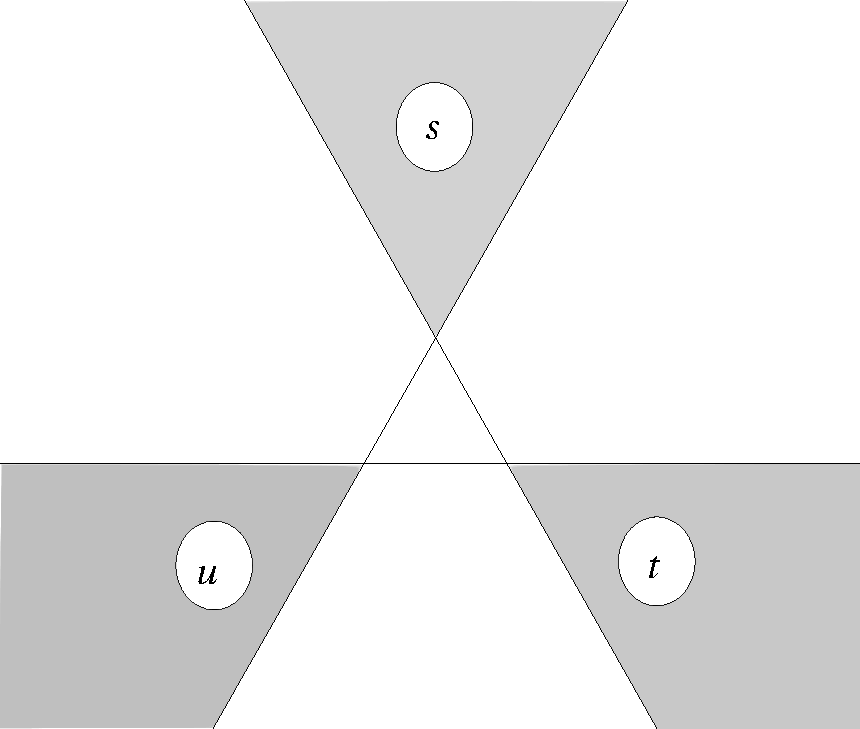
\includegraphics[width=7.225cm]{Imagenes/figurastesis/canalesfisicos.pdf}
\caption{El diagrama de  Mandelstam que muestra las regiones f\'isicas (regiones sombreadas) de los canales $s$, $t$, y $u$ para masas iguales.}
\label{figregfiscas}
\end{minipage}
&
\begin{minipage}[r]{7.225cm}
las relaciones inversas son:
%\begin{miscajax}
\begin{equation}\label{ecu2_20}
s=4(|\pmb{p}|^2+m)
\end{equation}
\begin{equation}
t=-2|\pmb{p}|^2(1-\cos\theta)\label{ecu2_21}.
\end{equation}
%\end{miscajax}
Usando las ecuaciones (\ref{ecu2_16}), (\ref{ecu2_20}) y (\ref{ecu2_21}) para masas iguales, podemos obtener para $u$, la siguiente expresi\'on:
%\begin{miscajax}
\begin{equation}
u=-2|\pmb{p}|^2(1+\cos\theta),
\end{equation}
%\end{miscajax}
Los dominios f\'isicos  de los canales $s$, $t$ y $u$, para masas iguales, se representan en la figura \ref{figregfiscas} (regiones sombreadas). 
\end{minipage}
\end{tabular}
\end{figure}
\subsection*{Secci\'on eficaz diferencial el\'astica}
La expresi\'on para  secci\'on eficaz diferencial el\'astica en t\'erminos de las variables invariantes de  Mandelstam para masas iguales es:
\begin{equation}\label{ecu2_27}
\frac{d\sigma_{el}}{dcos\theta}=\frac{1}{32\pi s}|A(s,t)|^2\ \ \ \textup{si la amplitud $A(s,t)$ es independinte de} \ \ \phi
\end{equation}
Diferenciando la ecuaci\'on (\ref{ecu2_19}) obtenemos:
\begin{equation}\label{ecu2_28}
d\cos\theta=\frac{2}{s-4m^2}dt
\end{equation}
A partir de  (\ref{ecu2_28}) y (\ref{ecu2_27}) se tiene:
\begin{equation}\label{ecu2_29}
\frac{d\sigma_{el}}{dt}=\frac{1}{64\pi s |\pmb{p}|^2}|A(s,t)|^2,
\end{equation}
y el teorema \'optico es: \cite{varone,donachie}
\begin{equation}\label{ecu2_30}
\sigma_{tot}=\frac{1}{2|\pmb{p}|\sqrt{s}}\textup{ Im}[A(s,t=0)]\ \ \textup{teorema \'optico}
\end{equation}
\subsection*{La expansi\'on para ${\pmb A\pmb(\pmb s\pmb ,\pmb t\pmb)}$ en ondas parciales}
Al igual que en la secci\'on (\ref{seccion2_3}), tambi\'en aqu\'i podemos expandir la amplitud de dispersi\'on $A(s,t)$ en ondas  parciales, esto es:
\begin{equation}\label{ecuqq2_1}
A(s,t(s,z))=\sum^{\infty}_{l=0}(2l+1) A_{l}(s)P_l(z),
\end{equation}
con
$t=t(s,z)$ y  $z=\cos\theta=1+\frac{2t}{s-4m^2}$.
La amplitud de onda parcial $A_l(s)$ es \cite{donachie}:\newpage
\begin{equation}\label{ecuqq2_2}
A_l(s)=\frac{1}{2}\int^{+1}_{-1}dzP_l(z)A(s,t(s,z))
\end{equation}
La ecuaci\'on (\ref{ecuqq2_2}) se obtiene de (\ref{ecuqq2_1}) haciendo uso de la relaci\'on de ortogonalidad de los polinomios de Legendre$P_l(z)$ :
\begin{equation}
\int^{+1}_{-1}dzP_{l}(z)P_{m}(z)=\frac{2}{2l+1}\delta_{ml}
\end{equation}
\subsection*{Interacciones a bajos valores de  t}
En dispersiones de protones cargados, las interacciones de Coulomb y nuclear, son las que contribuyen a la amplitud de dispersi\'on $f$. 
La amplitud de Coulomb ($f_c$) se obtiene a partir de la ecuaci\'on de Rutherford (se define $p\equiv|\pmb{p}|$ ): 
\begin{equation}
f_c=\frac{2p\alpha G^2(t)}{|t|},\ \ \  \hslash=c=1,
\end{equation}
donde $G(t)$ es el factor de forma electromagn\'etico del prot\'on. El signo ($+$) es para colisiones antiprot\'on-prot\'on y el ($-$) para colisiones prot\'on-prot\'on, $\alpha$ es la constante de estructura fina. La amplitud  nuclear $f_n$ para valores de $|t|<0\textup{.}1$ GeV$^2$ se puede expresar como  \cite{carlosavila}:
\begin{equation}
f_n=\frac{p\sigma_{tot}(\rho+i)\exp(-B|t|/2)}{4\pi},
\end{equation}
donde $B$ es el par\'ametro de pendiente nuclear, $\sigma_{tot}$ est\'a dada por el teorema \'optico y \begin{equation}\label{ecu2_33}
\rho \equiv \frac{\textup{Re}(f_n(t=0))}{\textup{Im}f_n(t=0)}
\end{equation}
De este modo la amplitud de dispersi\'on completa  es:
\begin{equation}\label{ecu2_34}
f=f_c+f_n \exp(\pm\alpha\phi(t))
\end{equation}
En la ecuaci\'on (\ref{ecu2_34}) $\alpha\phi$ es la diferencia de fase entre $f_c$ y $f_n$ y \begin{equation}
\phi(t)=\ln\left(\frac{0\textup{.}08}{|t|}\right)-0\textup{.}577
\end{equation}
Aqu\'i la secci\'on eficaz diferencial el\'astica viene dada por:
\begin{equation}\label{ecu2_36}
\frac{d\sigma_{el}}{dt}=\frac{\pi}{p^2}|f^2|
\end{equation}
De las ecuaciones (\ref{ecu2_29}) y (\ref{ecu2_36})
se puede concluir que:
\begin{equation*}
A(s,t)=8\pi\sqrt{s}f(t)
\end{equation*}
Remplazando en (\ref{ecu2_30}) obtenemos:
\begin{equation}
\sigma_{tot}=\frac{4\pi}{p}\textup{Im}[f(t=0)]
\end{equation}
En colisiones prot\'on-prot\'on, $\sigma_{tot}$  corresponde al \'area efectiva del prot\'on y provee informaci\'on de su tama\~no, el cual depende de la din\'amica del proceso de colisi\'on.\newpage

\sp La secci\'on eficaz diferencial el\'astica es:
\begin{align}\label{ecu2_38}
\frac{d\sigma_{el}}{dt}=\frac{d\sigma_{c}}{dt}+\frac{d\sigma_{inter}}{dt}+\frac{d\sigma_n}{dt},
\end{align}
donde
\begin{align}\label{ecu2_39}
\nonumber \frac{d\sigma_{c}}{dt}&=\frac{4\pi\alpha^2 G^4(t)}{|t|^2}\\
\nonumber \frac{d\sigma_{inter}}{dt}&=\pm\frac{\alpha(\rho\mp\alpha\phi)G^2(t)\sigma_{tot}}{|t|}\exp[-B|t|/2]\\
\frac{d\sigma_n}{dt}&=\frac{(1+\rho^2)\sigma^2_{tot}}{16\pi}\exp[-B|t|]
\end{align}
En la ecuaci\'on (\ref{ecu2_38}), el t\'ermino  $\frac{d\sigma_{inter}}{dt}$, se debe a la interferencia entre las amplitudes de dispersi\'on nuclear y coulomb que tambi\'en contribuyen a la secci\'on eficaz diferencial el\'astica \cite{carlosavila}. La dispersi\'on de Coulomb domina a valores muy bajos de $|t|$, por ejemplo, para una energ\'ia de 7 TeV, su contribuci\'on empieza a ser m\'axima para cuando $|t|<$0.0001 GeV$^2$ aproximadamente. Mientras que la contribuci\'on de la dispersi\'on nuclear empieza a ser  m\'axima para cuando $|t|>0.005$ GeV$^2$ aproximadamente, esto se puede apreciar en la figura \ref{figurasavila} \cite{carlosavila}.
\begin{figure}[H]
\centering
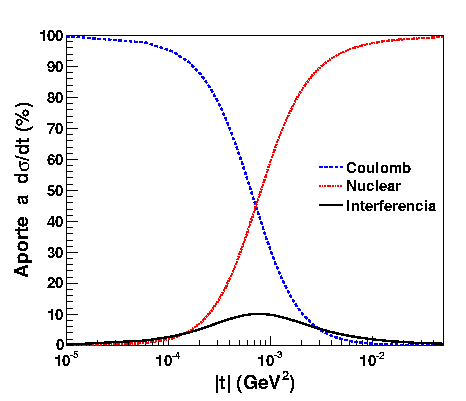
\includegraphics[width=8cm]{Imagenes/figurastesis/151-794-1-SM.pdf}
\caption{Aporte porcentual a $d\sigma/dt$ de la amplitud de dispersi\'on de Coulomb, nuclear e interferencia nuclear-Coulomb}.
\label{figurasavila}
\end{figure}
